% ============================================================
% DKU Academic Poster Template
% Matches SW-Poster-Templates-04.-PPT.pptx branding
% Paper size: A0 portrait (841mm x 1189mm)
%
% SETUP:
%   1. Rename logo:  cp "DKU Logo_Vertical _2_.png" DKU_logo.png
%   2. Compile:  latexmk main.tex  (uses pdflatex)
%   3. Requires beamerposter:  tlmgr install beamerposter
% ============================================================
\documentclass[10pt,final]{beamer}

% scale=1 → A0 default normalsize ≈ 25pt (standard for A0 posters)
% Using 10pt base class keeps fp arithmetic integer-friendly
\usepackage[size=a0,orientation=portrait,scale=1]{beamerposter}
\usepackage[T1]{fontenc}
% Arial substitute: Helvetica (visually identical at poster resolution)
\usepackage[scaled]{helvet}
\renewcommand{\familydefault}{\sfdefault}
\usepackage{graphicx}
\usepackage{xcolor}
\usepackage{booktabs}
\usepackage{amsmath,amssymb}
\usepackage{array}

\graphicspath{{./}{../paper/figures/}}

% ---- DKU Brand Colors ----
\definecolor{DKUnavy}{HTML}{17375E}
\definecolor{DKUlightblue}{HTML}{BDD7EE}
\definecolor{DKUmidblue}{HTML}{2E75B6}
\definecolor{DKUgreen}{HTML}{1F6B2E}

% ---- Beamer Color Setup ----
\setbeamercolor{headline}{bg=DKUnavy,fg=white}
\setbeamercolor{footline}{bg=DKUnavy,fg=white}
\setbeamercolor{separation line}{bg=DKUlightblue}
\setbeamercolor{structure}{fg=DKUnavy}
\setbeamercolor{normal text}{fg=black,bg=white}
\setbeamercolor{block title}{fg=white,bg=DKUnavy}
\setbeamercolor{block body}{fg=black,bg=white}
\setbeamercolor{block title alerted}{fg=white,bg=DKUmidblue}
\setbeamercolor{block body alerted}{fg=black,bg=DKUlightblue!30}
\setbeamercolor{block title example}{fg=white,bg=DKUgreen}
\setbeamercolor{block body example}{fg=black,bg=DKUgreen!10}
\setbeamercolor{item}{fg=DKUnavy}
\setbeamercolor{subitem}{fg=DKUmidblue}

% ---- Font Sizes ----
% Block section headings: 44pt (per DKU template)
% Poster main title:      72pt nominal; reduced to 58pt so the long title
%                         wraps cleanly on 0.65\paperwidth (~55cm)
\newcommand{\blocktitlefont}{\fontsize{44}{52}\selectfont\bfseries}
\newcommand{\headertitlefont}{\fontsize{58}{68}\selectfont\bfseries}
\newcommand{\headerauthorfont}{\fontsize{34}{42}\selectfont}
\newcommand{\headerinstitfont}{\fontsize{26}{32}\selectfont}

\setbeamerfont{block title}{size=\normalsize,series=\bfseries}
\setbeamerfont{block body}{size=\normalsize}
\setbeamertemplate{navigation symbols}{}
\setbeamertemplate{itemize item}{\color{DKUnavy}\rule{0.55em}{0.55em}}
\setbeamertemplate{itemize subitem}{\color{DKUmidblue}$\blacktriangleright$}

% ---- Header ----
% \parbox forces text wrapping for the long title.
% All elements stay in horizontal mode; no \vspace after minipages.
\setbeamertemplate{headline}{%
  \begin{beamercolorbox}[wd=\paperwidth,ht=13cm,dp=0.6cm]{headline}%
    \vspace{0.7cm}\par%
    \noindent\hspace{1.0cm}%
    \raisebox{-3.5cm}{\includegraphics[width=0.10\paperwidth]{DKU_logo}}%
    \hfill%
    \parbox{0.64\paperwidth}{%
      \centering%
      {\headertitlefont\color{white}\inserttitle\par}%
      \vspace{0.45cm}%
      {\headerauthorfont\color{DKUlightblue}\insertauthor\par}%
      \vspace{0.2cm}%
      {\headerinstitfont\color{DKUlightblue!85}\insertinstitute\par}%
    }%
    \hfill%
    \raisebox{-3.5cm}{\includegraphics[width=0.10\paperwidth]{DKU_logo}}%
    \hspace{1.0cm}%
  \end{beamercolorbox}%
  % Light blue separator
  \begin{beamercolorbox}[wd=\paperwidth,ht=0.6cm,dp=0]{separation line}
  \end{beamercolorbox}%
}

% ---- Footer ----
\setbeamertemplate{footline}{%
  \begin{beamercolorbox}[wd=\paperwidth,ht=0.6cm,dp=0]{separation line}
  \end{beamercolorbox}%
  \begin{beamercolorbox}[wd=\paperwidth,ht=2.4cm,dp=0.7cm,center]{footline}%
    \vspace{0.5cm}%
    {\fontsize{28}{34}\selectfont\color{white}%
      Duke Kunshan University
      \enspace$\cdot$\enspace
      Division of Natural and Applied Sciences
      \enspace$\cdot$\enspace
      Signature Work, Class of 2026%
    }%
  \end{beamercolorbox}%
}

% ---- Block Template ----
% colsep=0.3cm gives padding around title text without overflowing the box
\setbeamertemplate{block begin}{%
  \vspace{0.35cm}%
  \begin{beamercolorbox}[wd=\linewidth,colsep=0.3cm]{block title}%
    \blocktitlefont\insertblocktitle%
  \end{beamercolorbox}%
  \begin{beamercolorbox}[wd=\linewidth,colsep=0.3cm,colsep*=0.3cm]{block body}%
    \usebeamerfont{block body}%
}
\setbeamertemplate{block end}{%
  \end{beamercolorbox}%
}

\setbeamertemplate{block alerted begin}{%
  \vspace{0.35cm}%
  \begin{beamercolorbox}[wd=\linewidth,colsep=0.3cm]{block title alerted}%
    \blocktitlefont\insertblocktitle%
  \end{beamercolorbox}%
  \begin{beamercolorbox}[wd=\linewidth,colsep=0.3cm,colsep*=0.3cm]{block body alerted}%
    \usebeamerfont{block body}%
}
\setbeamertemplate{block alerted end}{%
  \end{beamercolorbox}%
}

\setbeamertemplate{block example begin}{%
  \vspace{0.35cm}%
  \begin{beamercolorbox}[wd=\linewidth,colsep=0.3cm]{block title example}%
    \blocktitlefont\insertblocktitle%
  \end{beamercolorbox}%
  \begin{beamercolorbox}[wd=\linewidth,colsep=0.3cm,colsep*=0.3cm]{block body example}%
    \usebeamerfont{block body}%
}
\setbeamertemplate{block example end}{%
  \end{beamercolorbox}%
}

% ============================================================
% Document Metadata
% ============================================================
\title{AI Code Quality Auto-Evaluation: A Diff-Based Agentic Workflow for SOLID Principle Violation Detection}
\author{Jiahe (Jay) Chen \enspace$\cdot$\enspace Mentor: Prof.\ Jiacheng Shen}
\institute{Duke Kunshan University \enspace$\cdot$\enspace Division of Natural and Applied Sciences \enspace$\cdot$\enspace Class of 2026}

% ============================================================
\begin{document}
\begin{frame}[t]
  \vspace{1.0cm}

  \begin{columns}[T]
    \hspace{1.2cm}

    % =========================================================
    % COLUMN 1 — Background & Dataset & Overall Results
    % =========================================================
    \begin{column}{0.29\paperwidth}

      \begin{block}{Introduction \& Motivation}
        Modern software increasingly relies on LLMs for code generation.
        Ensuring adherence to \textbf{SOLID design principles} is critical
        but \textbf{manual evaluation does not scale} to production codebases.
        We automate SOLID violation detection using a diff-based agentic workflow.
      \end{block}

      \begin{block}{SOLID Principles}
        \begin{itemize}
          \item \textbf{S}ingle Responsibility --- one reason to change
          \item \textbf{O}pen / Closed --- open for extension, closed for modification
          \item \textbf{L}iskov Substitution --- subtypes substitutable for base types
          \item \textbf{I}nterface Segregation --- prefer many specific interfaces
          \item \textbf{D}ependency Inversion --- depend on abstractions
        \end{itemize}
      \end{block}

      \begin{block}{Research Questions}
        \begin{enumerate}
          \item Can LLMs reliably detect SOLID violations in real-world code diffs?
          \item Does a diff-based agentic approach outperform single-pass evaluation?
          \item How does performance vary across violation types and difficulty levels?
        \end{enumerate}
      \end{block}

      \begin{block}{Dataset}
        \begin{itemize}
          \item \textbf{240 code diffs} from open-source Python repositories
          \item Expert-annotated; 48 examples per SOLID class
          \item Difficulty: Easy (33 LOC), Moderate (140 LOC), Hard (306 LOC)
        \end{itemize}
      \end{block}

      \begin{block}{Results: Overall Accuracy}
        \begin{center}
          
\includegraphics[width=0.95\linewidth]{paper_fig_overall}
        \end{center}
        Diff Eval achieves \textbf{87.9\%}, outperforming Single Agent (70.0\%)
        and Two Agent (55.8\%) by \textbf{+17.9 pp}.
      \end{block}

      \begin{block}{Results: Accuracy by Difficulty}
        \begin{center}
          
\includegraphics[width=0.95\linewidth]{paper_fig_difficulty}
        \end{center}
        Diff Eval maintains $\geq$80\% even on hard examples (306 LOC).
      \end{block}

    \end{column}

    \hspace{1.0cm}

    % =========================================================
    % COLUMN 2 — Architecture & Methodology
    % =========================================================
    \begin{column}{0.29\paperwidth}

      \begin{block}{System Architecture}
        \begin{center}
          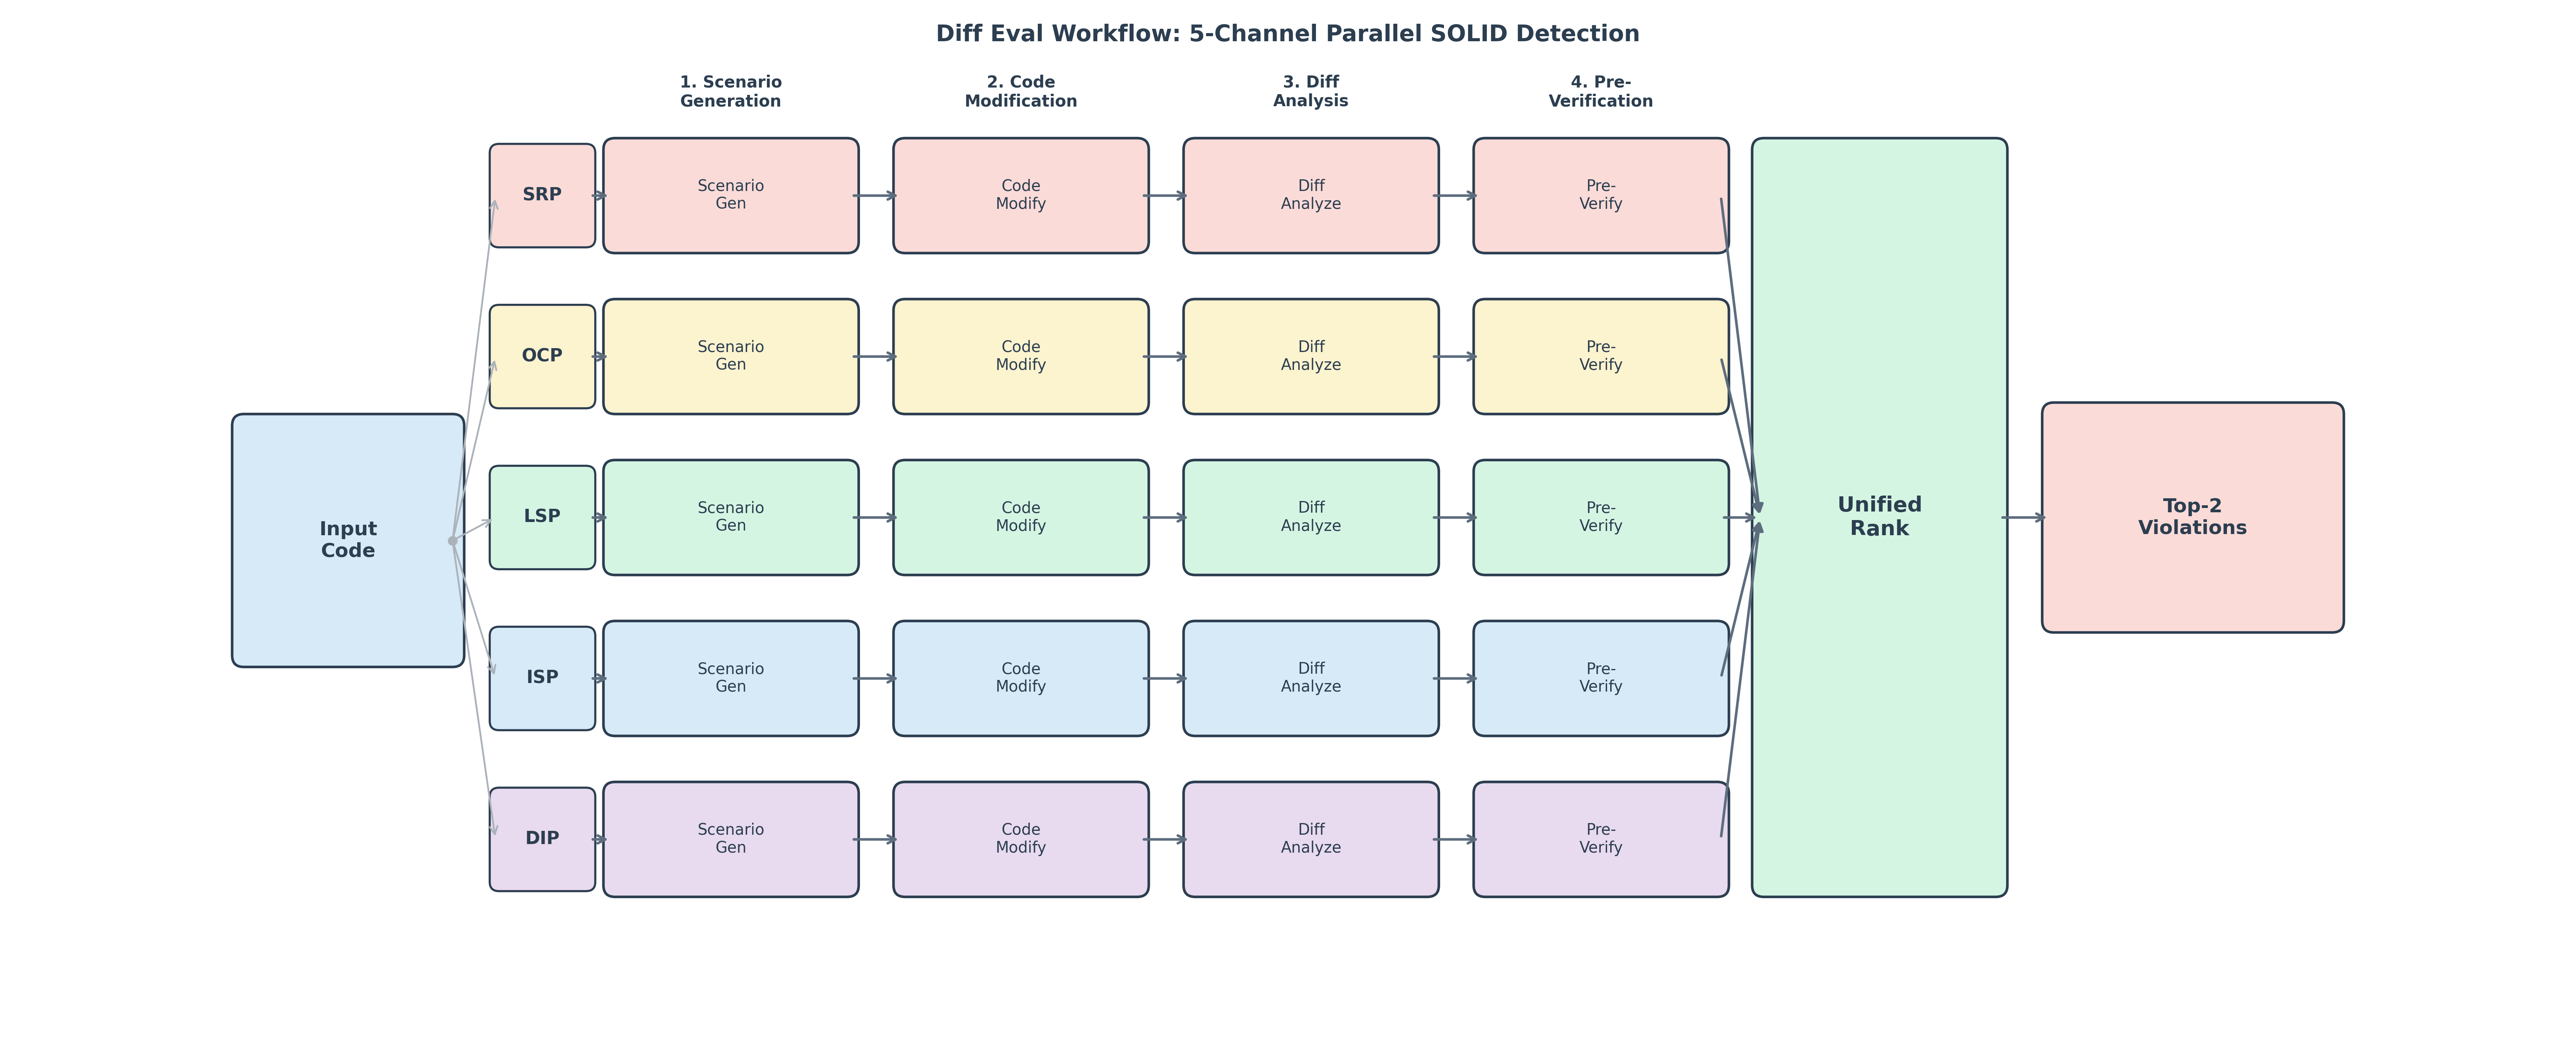
\includegraphics[width=0.97\linewidth]{architecture_diff_eval}
        \end{center}
        \vspace{0.1cm}
        Five parallel sub-agents each specialise in one SOLID principle.
        Each channel independently generates scenarios, modifies code, analyzes
        the resulting diff, and pre-verifies its verdict before a unified ranking
        resolves conflicts.
      \end{block}

      \begin{block}{Diff-Based Evaluation Pipeline}
        \begin{enumerate}
          \item \textbf{Scenario Generation} — Enumerate plausible violation
            scenarios for the target principle.
          \vspace{0.2cm}
          \item \textbf{Code Modification} — Minimally transform code to embody the violation
          \item \textbf{Diff Analysis} — Confirm structural signals in the resulting diff
          \item \textbf{Pre-Verification} — Self-consistency check before unified ranking
        \end{enumerate}
      \end{block}

      \begin{block}{Why Diff-Based?}
        \begin{itemize}
          \item Focuses on \emph{changes} introduced by a commit, not pre-existing style
          \item Reduces false positives; mirrors pull-request code review
          \item Provides fine-grained, explainable output per principle
        \end{itemize}
      \end{block}

      \begin{block}{Baseline Comparisons}
        \begin{center}
          \renewcommand{\arraystretch}{1.5}
          \begin{tabular}{lccc}
            \toprule
            \textbf{Method} & \textbf{Agents} & \textbf{Diff} & \textbf{Accuracy} \\
            \midrule
            Single Agent    & 1  & \texttimes & 70.0\% \\
            Two Agent       & 2  & \texttimes & 55.8\% \\
            \textbf{Diff Eval} & \textbf{5} & \checkmark & \textbf{87.9\%} \\
            \midrule
            Random Baseline & — & — & 40.0\% \\
            \bottomrule
          \end{tabular}
        \end{center}
      \end{block}

      \begin{block}{Accuracy by SOLID Principle}
        \begin{center}
          
\includegraphics[width=0.97\linewidth]{paper_fig_violation}
        \end{center}
        \vspace{-0.2cm}
        ISP (98\%) and SRP (96\%) reach near-perfect accuracy. LSP (81\%)
        remains the most challenging, reflecting its subtle type-substitution semantics.
      \end{block}

    \end{column}

    \hspace{1.0cm}

    % =========================================================
    % COLUMN 3 — Confusion Matrix, Conclusions, References
    % =========================================================
    \begin{column}{0.29\paperwidth}

      \begin{block}{Confusion Matrix — Diff Eval}
        \begin{center}
          
\includegraphics[width=0.90\linewidth]{paper_fig_confusion}
        \end{center}
        \vspace{-0.1cm}
        Strong diagonal dominance confirms the model reliably distinguishes
        all five SOLID classes. OCP-to-SRP confusion (23\%) is the main
        error mode, reflecting structural overlap between the two principles.
      \end{block}

      \begin{alertblock}{Key Findings}
        \begin{itemize}
          \item Diff-based agentic workflow achieves \textbf{87.9\% accuracy},
            far above the 40\% random baseline
          \item Specialised per-principle agents are critical: the generalist
            Two Agent baseline drops \textbf{14 pp} vs.\ Single Agent
          \item Performance is \textbf{robust to code length} --- hard examples
            (306 LOC) still reach 80\%
          \item ISP and SRP are easiest; \textbf{LSP remains the hardest} class
            across all methods
        \end{itemize}
      \end{alertblock}

      \begin{block}{Conclusion}
        We demonstrate that a diff-based multi-agent LLM pipeline can
        \textbf{automate SOLID violation detection at scale}, matching expert-level
        precision on a diverse benchmark.

        \vspace{0.3cm}
        The diff-based framing is the decisive design choice: by constraining
        analysis to code changes, the system focuses on violations
        \emph{introduced} by a commit, eliminating noise and yielding
        highly interpretable, actionable reports.
      \end{block}

      \begin{block}{Future Work}
        \begin{itemize}
          \item \textbf{CI/CD integration} — real-time SOLID checks on pull requests
          \item Multi-language support beyond Python (Java, TypeScript)
          \item Extension to broader design pattern detection
          \item Fine-tuning smaller models on the annotated benchmark
        \end{itemize}
      \end{block}

      \begin{block}{Acknowledgements}
        This work was conducted under the supervision of Prof.\ Jiacheng Shen,
        Division of Natural and Applied Sciences, Duke Kunshan University.
        The author thanks the DKU Data Science program for computational
        resources and peer reviewers for feedback.
      \end{block}

      \begin{block}{References}
        {\fontsize{22}{27}\selectfont
        \begin{enumerate}
          \item Martin, R.C.\ (2000). \textit{Design Principles and Design Patterns}.
            Object Mentor.
          \item Wei et al.\ (2022). Chain-of-Thought Prompting. \textit{NeurIPS}.
          \item Chen et al.\ (2021). Evaluating Large Language Models Trained
            on Code. \textit{arXiv:2107.03374}.
          \item Yao et al.\ (2023). ReAct: Synergizing Reasoning and Acting
            in Language Models. \textit{ICLR}.
        \end{enumerate}
        }
      \end{block}

    \end{column}

    \hspace{1.2cm}
  \end{columns}

\end{frame}
\end{document}